% Github link to this file:
% https://github.com/yungyuc/r-isildur/blob/master/note/isildur_note.tex

% Overleaf document link:
% https://www.overleaf.com/project/6093eb9176f838fa8c3da086

\documentclass{isildur}
%\documentclass[aps,pra,preprint]{revtex4-2}

%\usepackage{lmodern}

\usepackage[printwatermark]{xwatermark}
\newwatermark[allpages,color=black!15,angle=55,scale=5,xpos=0,ypos=0]%
{DRAFT}

%\doublespacing
\linespread{1.2}

\title{
%
High-Order Harmonic Generation by Using the CESE Method
%
}

\author{
%
Tsin-Fu Jiang and Yung-Yu Chen
%
}

\date{July 2021}

\begin{document}

\maketitle

\tableofcontents

%%%%%%%%%%%%%%%%%%%%%%%%%%%%%%%%%%%%%%%%%%%%%%%%%%%%%%%%%%%%%%%%%%%%%%%%%%
%%
\chapter{Introduction}
\label{c:intro}
%%
%%%%%%%%%%%%%%%%%%%%%%%%%%%%%%%%%%%%%%%%%%%%%%%%%%%%%%%%%%%%%%%%%%%%%%%%%%

A proposal to investigate the high-order harmonic generations (HHG) by using
the CESE method.

\section{The Space-Time Conservation Element and Solution Element Method}

There are several possible quantum mechanical applications by the conservation
element and solution element (CESE) method.  We may try the first study on the
most important one, the HHG.  The HHG first appeared in the ’80s with intense
laser pulse on inert atomic gas.  By using the laser with frequency $\omega$,
the harmonics of integer multiples order $n\omega$ up to thousands can be
generated.

For example, with the infrared laser, near X-ray light can be generated on
desktop facility without a traditional X-ray room.

With the progress of laser technology, the pulse duration of attosecond scale
was developed in 2000.  The extreme time scale is in the order of atomic
electron motion and probing the real-time electron dynamics is an emerging new
area of quantum science.  There are new findings with different types of pulses
on targets such as atoms, molecules, and solid from time to time.

Under the interaction of intense light, atomic valence electron absorbs photons
from the field.  Classically, the electric field drives the electron.  The
laser oscillates at frequency, it drives the electron forward and backward,
when the electron moves near the nucleus, the electron can interacts with the
nucleus, jump to the ground state and releases absorbed photons.  So the
emission mechanism happens near the nucleus, a finite space is enough for
simulation.  But the electron will move to far distance, the non-reflecting
boundary is critical and necessary to keep from the interference from the
numerical artifacts.

There are many theoretical methods for the HHG study.  To my knowledge, the
CESE method would be the best one.  No papers reported with this method so far,
because the CESE method is not well known by the researchers in the field.

Physically, the HHG comes from the oscillation of electron which can be
described by the dipole functions. We give an initial state and solve the
dipole functions.  After the calculation, tale Fourier transform of the dipole
function into frequency spectra and obtain the HHG.  The governing equation is
the time-dependent Schrödinger equation (TDSE).

%%%%%%%%%%%%%%%%%%%%%%%%%%%%%%%%%%%%%%%%%%%%%%%%%%%%%%%%%%%%%%%%%%%%%%%%%%
%%
\chapter{Governing Equations}
\label{c:goveq}
%%
%%%%%%%%%%%%%%%%%%%%%%%%%%%%%%%%%%%%%%%%%%%%%%%%%%%%%%%%%%%%%%%%%%%%%%%%%%

Time-dependent Schrödinger equation (TDSE):

\begin{align}
  i\frac{\partial \Psi(x, y, z, t)}{\partial t}
    &= -\frac{1}{2}\nabla^2\Psi + V(r)\Psi + H'(x, y, z, t)\Psi
    \label{e:tdse} \\
  r &= \sqrt{x^2+y^2+z^2} \nonumber \\
  V(r) &= \frac{-1}{r}
        - \frac{a_1e^{-a_2r}+a_3re^{-a_4r}+a_5e^{-a_6r}}{r} \\
  H' &= \mathbf{r}\cdot \mathbf{E}(t),
\end{align}

$\Psi$ is the wave function.  $V(r)$ is an atomic model potential.  $H'$ is the
interaction between the atomic electron and laser field in dipole
approximation.  Atomic units ($\hbar = e = m = 1$) were used.

After the development of dipole approximation, we may extend to non-dipole
approximation which is another research topic.  There are two classes of the
field.

\section{The Linearly Polarized Laser Pulse}

\begin{align}
  \mathbf{E}(t) &= {\hat z}E_0e^{-\alpha t^2}\cos(\omega t+\phi), \\
  H' &= zE_0e^{-\alpha t^2}\cos(\omega t+\phi),
\end{align}
%
$\alpha$ is to characterize the pulse duration and $\phi$ is called the
carrier-envelope-phase which is a constant.

\section{The Circularly Polarized Laser Pulse}

\begin{align}
  \mathbf{E}(t) &=
    \frac{E_0}{\sqrt 2}e^{-\alpha t^2}
    \left[
      {\hat x}\cos(\omega t+\phi)+{\hat y}\sin(\omega t+\phi)
    \right], \\
  H' &= \frac{E_0}{\sqrt 2}e^{-\alpha t^2}
    \left[
      x\cos(\omega t+\phi) + y\sin(\omega t+\phi)
    \right],
\end{align}
%
The circularly polarized case can be extended to elliptically polarized case
later.

The pulse duration is defined by $-\frac{\tau}{2}$ to $\frac{\tau}{2}$ where
$e^{-\alpha \tau^2/4}\sim 10^{-4,-5}$.  With a given initial state
$\Psi(x,y,x,t=-\frac{\tau}{2})$, time evolve the Eq.~(\ref{e:tdse}) to
$\frac{\tau}{2}$ with a finite space, keep the dipole functions at each time
step
%
\begin{align}
  \langle x(t) \rangle = \int x |\Psi(x,y,z,t)|^2 \dif x \dif y \dif z,
\end{align}
%
and $\langle y(t) \rangle, \langle z(t) \rangle$.  This part is done.

\section{Burnett's Problem}

The initial state is the ground state $\Psi_g(x)$ of the eigenvalue equation
%
\begin{align}
  \left[ -\frac{1}{2}\frac{\dif^2}{\dif x^2}-\frac{1}{\sqrt{x^2+1}} \right]
  \Psi(x) = \varepsilon \Psi(x).
\end{align}

1D TDSE: to solve the initial value problem with $\Psi(x,t=0)=\Psi_g(x)$:
%
\begin{align}
  i\frac{\partial \Psi(x,t)}{\partial t} &=
    \left[
      -\frac{1}{2}\partial^2_{x} - \frac{1}{\sqrt{x^2+1}} + xE(t)\sin\omega t
    \right]\Psi, \\
  E(t) &= E_{0}\sin^2(\frac{\pi t}{T}) \\
  a(t) &= \langle \Psi(x,t)|\frac{x}{(1+x^2)^{3/2}}|\Psi(x,t) \rangle
        + \langle \Psi(x,t)|\Psi(x,t) \rangle \cdot E(t)\sin\omega t.
    \label{e:a(t)}
\end{align}
%
Parameters:
%
\begin{itemize}

  \item wavelength $\lambda$ to frequency:
  $\omega \,\mathrm{(au)} = 45.5633525 / \lambda \,\mathrm{(nm)}, \,
  \omega \,\mathrm{(eV)} = \omega \,\mathrm{(au)}\, \times 27.21$.

  \item peak power to peak electric field $E_0$:
  $E_0(au)=\sqrt{\frac{(PeakPower) 10^{14}{W/cm^2}}{351.0}}$

  \item femtosecond (fs) to au: $\mathrm{fs} = \frac{100.0}{2.418884326505} =
  41.341 \,\mathrm{au}$.

\end{itemize}
%
In \cite{burnett_calculation_1992}, parameters in atomic units (au):
%
\begin{itemize}

  \item $\lambda=300\mathrm{nm}, \,\omega=0.151878 \,\mathrm{au}$,
  $\mathrm{cycle} = \mathrm{period} = \frac{2\pi}{\omega} = 41.37
  \,\mathrm{au}$.

  \item pulse duration $T=50$ fs =2067.07 au $\sim$ 50-cycle.

  \item peak power 2$\times 10^{14}W/cm^2, E_0=7.4851356\times 10^{-2}$;
  3.2$\times 10^{15}W/cm^2, E_0=0.30194$.

  \item try $x\in (-100,100)$, pulse duration  $T \in (0,2067.07)$, time
  marching step $\dif t=0.1$.  Adjust later for $\dif x, \dif t$.

  \item Fig.2 and Fig.4 are to calibrate.  Fig.2 is our acceleration function
  of Eq.~(\ref{e:a(t)}).  Fig.4 is obtained by use their Eq.(1) with the
  acceleration function of Eq.~(\ref{e:a(t)}).

Note that the asymptotic behavior $V(x)\rightarrow -1/|x|$, the range of $x$
must be large to keep a good representation of the system. For the case of
laser power intensity $3.2\times 10^{15} W/cm^2$, the electron has been ionized
much early before the end of pulse. We test the intensity $2\times 10^{14}
W/cm^2$ case only and calculated the acceleration function and its HHG
spectrum. ie, Fig.2a and Fig.4a in PRA45.3347.

\begin{figure}[htbp] \centering
\mbox{\rotatebox{-90}{\scalebox{0.5}[0.7]{
\includegraphics[width=\linewidth]{fig1a.eps}} }}
\caption{Acceleration function with x in [-100,100]. Green line is the norm vs time.
 }
\end{figure}
\begin{figure}[htbp]
\centering
\mbox{\rotatebox{-90}{\scalebox{0.5}[0.7]{
\includegraphics[width=\linewidth]{fig1b.eps}} }}
\caption{HHG spectrum with x in [-100,100].
 }
\end{figure}
\begin{figure}[htbp]
\centering
\mbox{\rotatebox{-90}{\scalebox{0.5}[0.7]{
\includegraphics[width=\linewidth]{fig2a.eps}} }}
\caption{Acceleration function with x in [-1500,1500]. The norm is 1 till the
end. It means wave function lies inside the range all the time.
 }
\end{figure}
\begin{figure}[htbp]
\centering
\mbox{\rotatebox{-90}{\scalebox{0.5}[0.7]{
\includegraphics[width=\linewidth]{fig2b.eps}} }}
\caption{HHG spectrum with x in [-1500,1500].
 }
\end{figure}
\begin{figure}[htbp]
\centering
\mbox{\rotatebox{-90}{\scalebox{0.5}[0.7]{
\includegraphics[width=\linewidth]{fig3a.eps}} }}
\caption{ Calculation by p-space method. Velocity and norm vs time.
 }
\end{figure}
\begin{figure}[htbp]
\centering
\mbox{\rotatebox{-90}{\scalebox{0.5}[0.7]{
\includegraphics[width=\linewidth]{fig3b.eps}} }}
\caption{HHG spectrum by p-space method.
 }
\end{figure}

Apparently, $ x\in[-100,100]$ is too small in range and results Figs.2.1,2.2
are not reliable.
%
During the development of CESE code, Figs.2.3 and 2.4 can be used for
comparison where 51200 grids in x were used. Since there is Fast Fourier
Transform routine, a job with 32768 time steps takes only a few minutes.
%
The Fig.2.6 is accurate, it takes time about 24 hours to finish a job. Hope to
parallelize the f90 version if necessary.

\end{itemize}

%%%%%%%%%%%%%%%%%%%%%%%%%%%%%%%%%%%%%%%%%%%%%%%%%%%%%%%%%%%%%%%%%%%%%%%%%%
%%
\clearpage
\addcontentsline{toc}{chapter}{Bibliography}
%%
%%%%%%%%%%%%%%%%%%%%%%%%%%%%%%%%%%%%%%%%%%%%%%%%%%%%%%%%%%%%%%%%%%%%%%%%%%

%\bibliographystyle{myunsrtnat} % no sort (order in appearance)
\bibliographystyle{myplainnat} % sort by author
\bibliography{isildur}

\end{document}

% vim: set et sw=2 ts=2 sts=2 tw=79:
